\section{Experiments}
\label{sec:experiments}

\subsection{Setup}
\label{sec:setup}

\paragraph{Model and training.} We train MAML with the Conv4 backbone (four $3{\times}3$ conv + BatchNorm + ReLU + $2{\times}2$ maxpool blocks) under Finn~\etal's original protocol~\cite{finn2017model}: inner-loop rate $\alpha{=}0.01$, Adam outer-loop rate $\beta{=}0.001$, $T_{\text{train}}{=}5$ / $T_{\text{test}}{=}10$ adaptation steps, meta-batch size 4, 60{,}000 meta-training iterations, 5-way 1-shot. All results use the converged checkpoint at $T{=}T_{\text{test}}$.

\paragraph{Datasets.} \emph{miniImageNet}~\cite{ravi2017optimization}: 100 ImageNet classes, 600 images each, 64/16/20 train/val/test split, our standard-difficulty control. \emph{tieredImageNet}~\cite{ren2018meta}: a larger, WordNet-hierarchy-split variant (608 classes, split at the 20/6/8 super-category level), whose semantically distant test classes make it our primary quantitative benchmark and the harder domain-shift setting. \emph{CUB-200-2011}~\cite{welinder2010caltech}: 200 fine-grained bird species ($\sim$60 images/class); its subtle inter-class differences make it a stress test for negative transfer and our OOD probe.

\paragraph{Protocol.} All three quantitative checks (\Cref{sec:biadt,sec:sanity}) run on $N{=}600$ sampled tieredImageNet meta-test tasks, with $\Delta M$ itself estimated per task via stratified bootstrap query sets (\Cref{sec:adaptation_gain}); CUB-200-2011 additionally supplies the OOD condition for the support-set sanity check. Across these 600 tasks we report mean $\pm$ MoE, the half-width of a 96\% bootstrap percentile confidence interval on the mean (10{,}000 resamples), and test \biadt significance with a one-sided one-sample $t$-test against zero. For qualitative analysis we run \fama on 600 further sampled cross-domain tasks each for miniImageNet$\to$CUB (\emph{mini2cub}) and tieredImageNet$\to$CUB (\emph{tiered2cub}).

\subsection{Quantitative Results}
\label{sec:quant_results}

\begin{table}[t]
\centering\small
\caption{\biadt on tieredImageNet ($N{=}600$ tasks): both directions are positive and significant (one-sided one-sample $t$-test against 0), confirming $\PhiFama$'s sign is causally linked to $\Delta M$.}
\label{tab:biadt}
\begin{tabular}{@{}lcc@{}}
\toprule
Metric & Mean $\pm$ MoE & $p$-value \\
\midrule
$\mathrm{ABC}_\downarrow$ & $0.186 \pm 0.109$ & $1.99{\times}10^{-4}$ \\
$\mathrm{ABC}_\uparrow$   & $0.289 \pm 0.122$ & $7.01{\times}10^{-7}$ \\
\bottomrule
\end{tabular}
\end{table}

\paragraph{\biadt (\Cref{tab:biadt}).} Both $\mathrm{ABC}_\downarrow$ and $\mathrm{ABC}_\uparrow$ are positive with $p<0.001$: deleting superpixels in either direction indicated by $\PhiFama$ shifts $\Delta M$ significantly faster than random deletion. $\mathrm{ABC}_\uparrow$ exceeds $\mathrm{ABC}_\downarrow$, i.e.\ the harmful-region signal separates from the random baseline more cleanly than the helpful-region signal. The relatively wide margins (\raise.17ex\hbox{$\scriptstyle\sim$}59\% of the mean for $\mathrm{ABC}_\downarrow$) are consistent with Conv4's coarse final feature grid: bilinear upsampling (\Cref{eq:branch_saliency}) from a low-resolution map blurs region boundaries and adds variance without changing the sign of the effect (\Cref{sec:limitations}).

\begin{table}[t]
\centering\small
\caption{Sanity checks on tieredImageNet ($N{=}600$ tasks; Spearman~/~Pearson correlation against the unperturbed $\PhiFama$, mean $\pm$ MoE). \textbf{Top:} cascading randomization of $\theta_0^b$ collapses to the noise floor as soon as the output-nearest block is destroyed. \textbf{Bottom:} all three $S_i$ interventions shift the map significantly below the near-1 correlation of a content-blind detector.}
\label{tab:sanity}
\begin{tabular}{@{}lcc@{}}
\toprule
\multicolumn{3}{@{}l}{\textit{(a) Cascading randomization of $\theta_0^{b}$}} \\
Destroyed block & Spearman & Pearson \\
\midrule
none (head only) & $0.085\pm.016$ & $0.087\pm.016$ \\
conv block 4      & $-0.010\pm.012$ & $-0.012\pm.012$ \\
conv block 3      & $-0.008\pm.012$ & $-0.007\pm.013$ \\
conv block 2      & $-0.013\pm.012$ & $-0.013\pm.012$ \\
conv block 1      & $-0.006\pm.012$ & $-0.005\pm.012$ \\
\midrule
\multicolumn{3}{@{}l}{\textit{(b) Intervention on $S_i$}} \\
Scenario & Spearman & Pearson \\
\midrule
OOD task mixing    & $0.330\pm.018$ & $0.340\pm.018$ \\
Label permutation  & $0.250\pm.023$ & $0.258\pm.024$ \\
Hard task (blur)   & $0.258\pm.016$ & $0.266\pm.016$ \\
\bottomrule
\end{tabular}
\end{table}

\paragraph{Randomizing $\theta_0$ (\Cref{tab:sanity}a).} Correlation collapses from $\approx\!0.09$ to $\approx\!0$ the instant the output-nearest block is randomized, then stays flat (all remaining blocks fall in $[-0.013,0.000]$) -- batch-norm sub-layers behave consistently with their paired conv layer at every depth. This step-function collapse could look like a resolution artifact of Conv4's shallow 5-level ladder, so we isolated it with a control: replacing $\Delta M$ in \Cref{eq:adaptation_gain} with the un-intervened contrast $\Delta M':=\mathbb{E}_{Q_i}[\mathcal{L}(Q_i,\theta_0)-\mathcal{L}(Q_i,\phi_T)]$ (\emph{any} adaptation vs.\ none, rather than free vs.\ frozen) reproduces the same cascading-randomization sweep as a \emph{smooth}, monotonic decay from $0.650$ (head only) to $0.075$ (deepest block) -- because a linear head can still exploit the generic edge/texture structure that even a randomly initialized conv stack produces, regardless of what $\theta_0^b$ actually learned. Per~\cite{adebayo2018sanity}, a gently-decaying map is the \emph{failure} signature, not the pass; \fama's two-branch subtraction (\Cref{eq:fama_final}) is precisely what cancels that architecture-only floor and leaves only the part that depends on $\theta_0^b$'s learned content, exactly as \Cref{prop:decomposition} predicts.

\paragraph{Intervening on $S_i$ (\Cref{tab:sanity}b).} All three interventions pull correlation down to $0.25$--$0.34$, well below what a content-blind map would show. Counter-intuitively, label permutation and hard-task blur perturb the map \emph{more} than OOD task mixing, even though OOD mixing looks like the more destructive edit. The reason is what each intervention corrupts: permutation and blur corrupt the \emph{supervisory signal} used at every one of the $T$ adjoint steps, compounding across the trajectory, whereas OOD mixing keeps each image-label pair internally consistent, so every local adaptation step remains locally "valid" even though the task as a whole is off-distribution -- compounded by Conv4 being shallow enough that CUB and tieredImageNet, despite being semantically disjoint, still share enough low-level texture statistics (centered subject, contrasting background) to activate similar early filters.

\subsection{Qualitative Case Studies}
\label{sec:qual_results}

\begin{figure}[t]
    \centering
    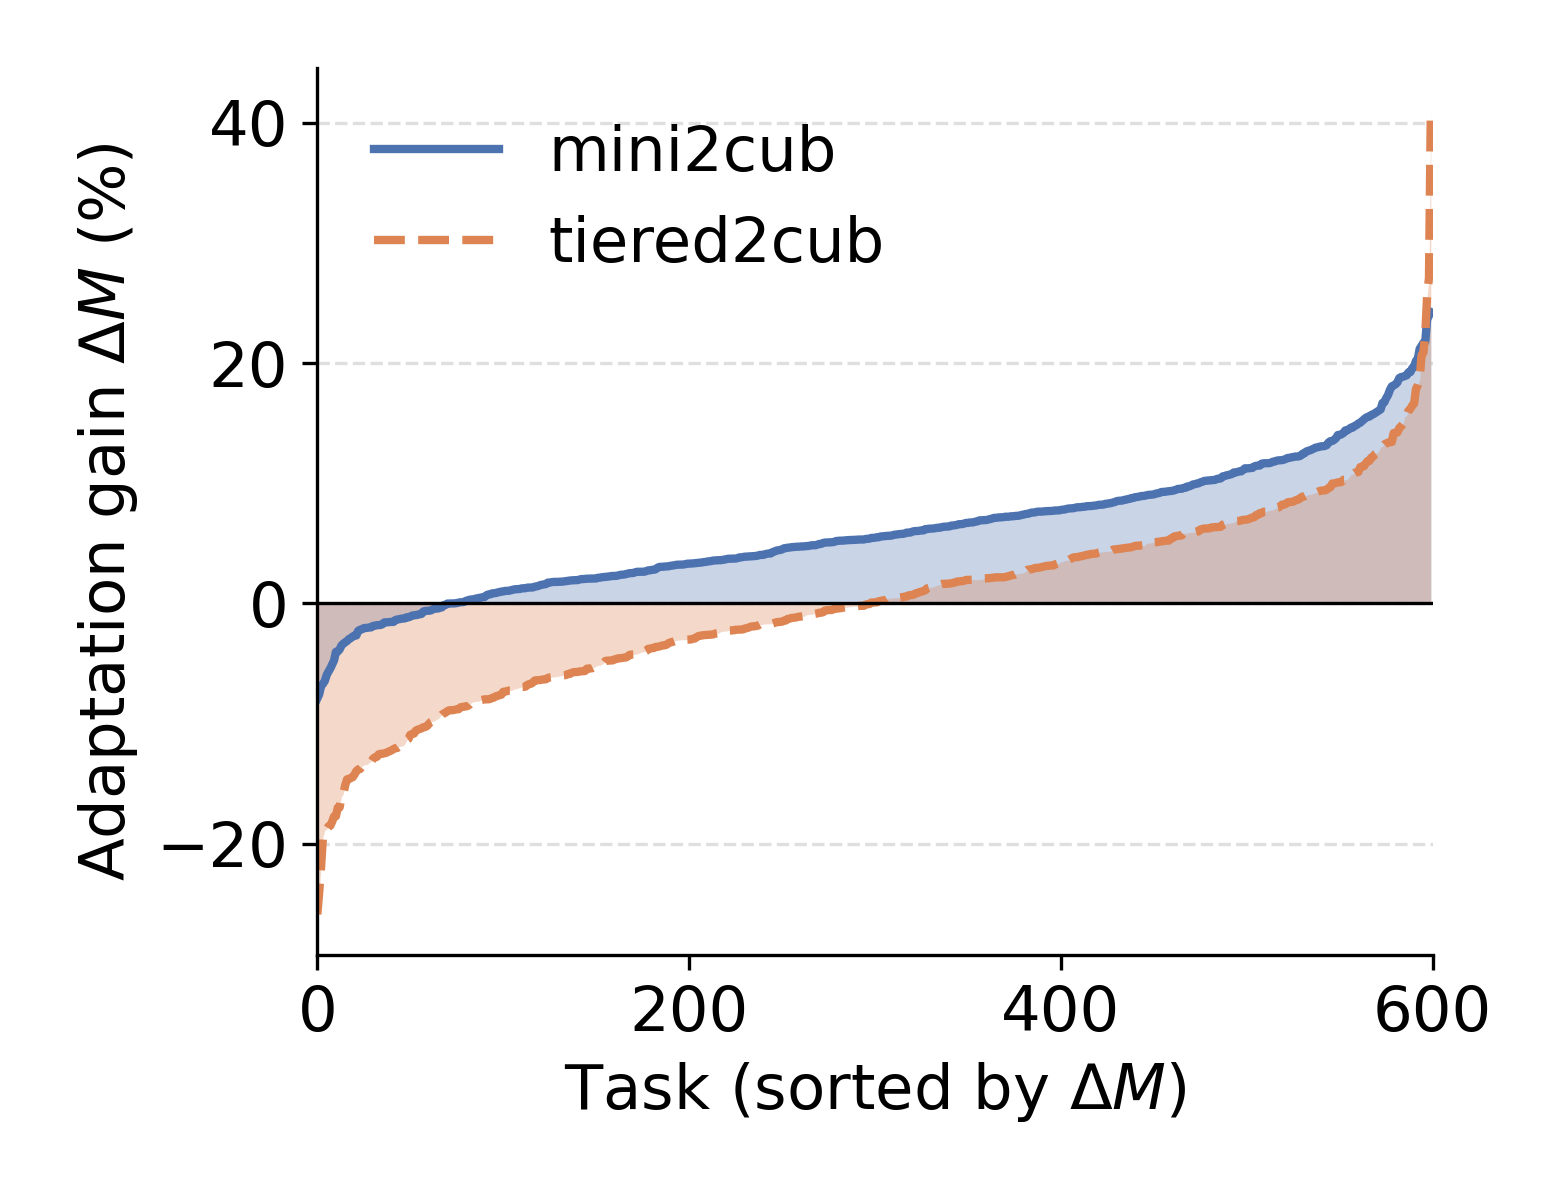
\includegraphics[width=\linewidth]{figures/delta_m_distribution.png}
    \caption{Sorted $\Delta M$ over 600 tasks per benchmark. tiered2cub is both wider (tails at $-25.88\%$/$+41.24\%$ vs.\ $-7.91\%$/$+24.24\%$) and far more often negative (49.7\% of tasks vs.\ 12.5\%), consistent with tieredImageNet's category-level split yielding broader but less fine-grained prior knowledge.}
    \label{fig:delta_m_dist}
\end{figure}

\Cref{fig:delta_m_dist} sorts $\Delta M$ over 600 sampled tasks for both cross-domain settings. tiered2cub is both wider and far more negative-heavy than mini2cub, matching tieredImageNet's coarser, category-level prior: it generalizes broadly but lacks the fine-grained specialization CUB's subtle inter-species boundaries require, so backbone adaptation becomes higher-variance -- swinging further in both directions depending on task content.

\begin{figure*}[t]
    \centering
    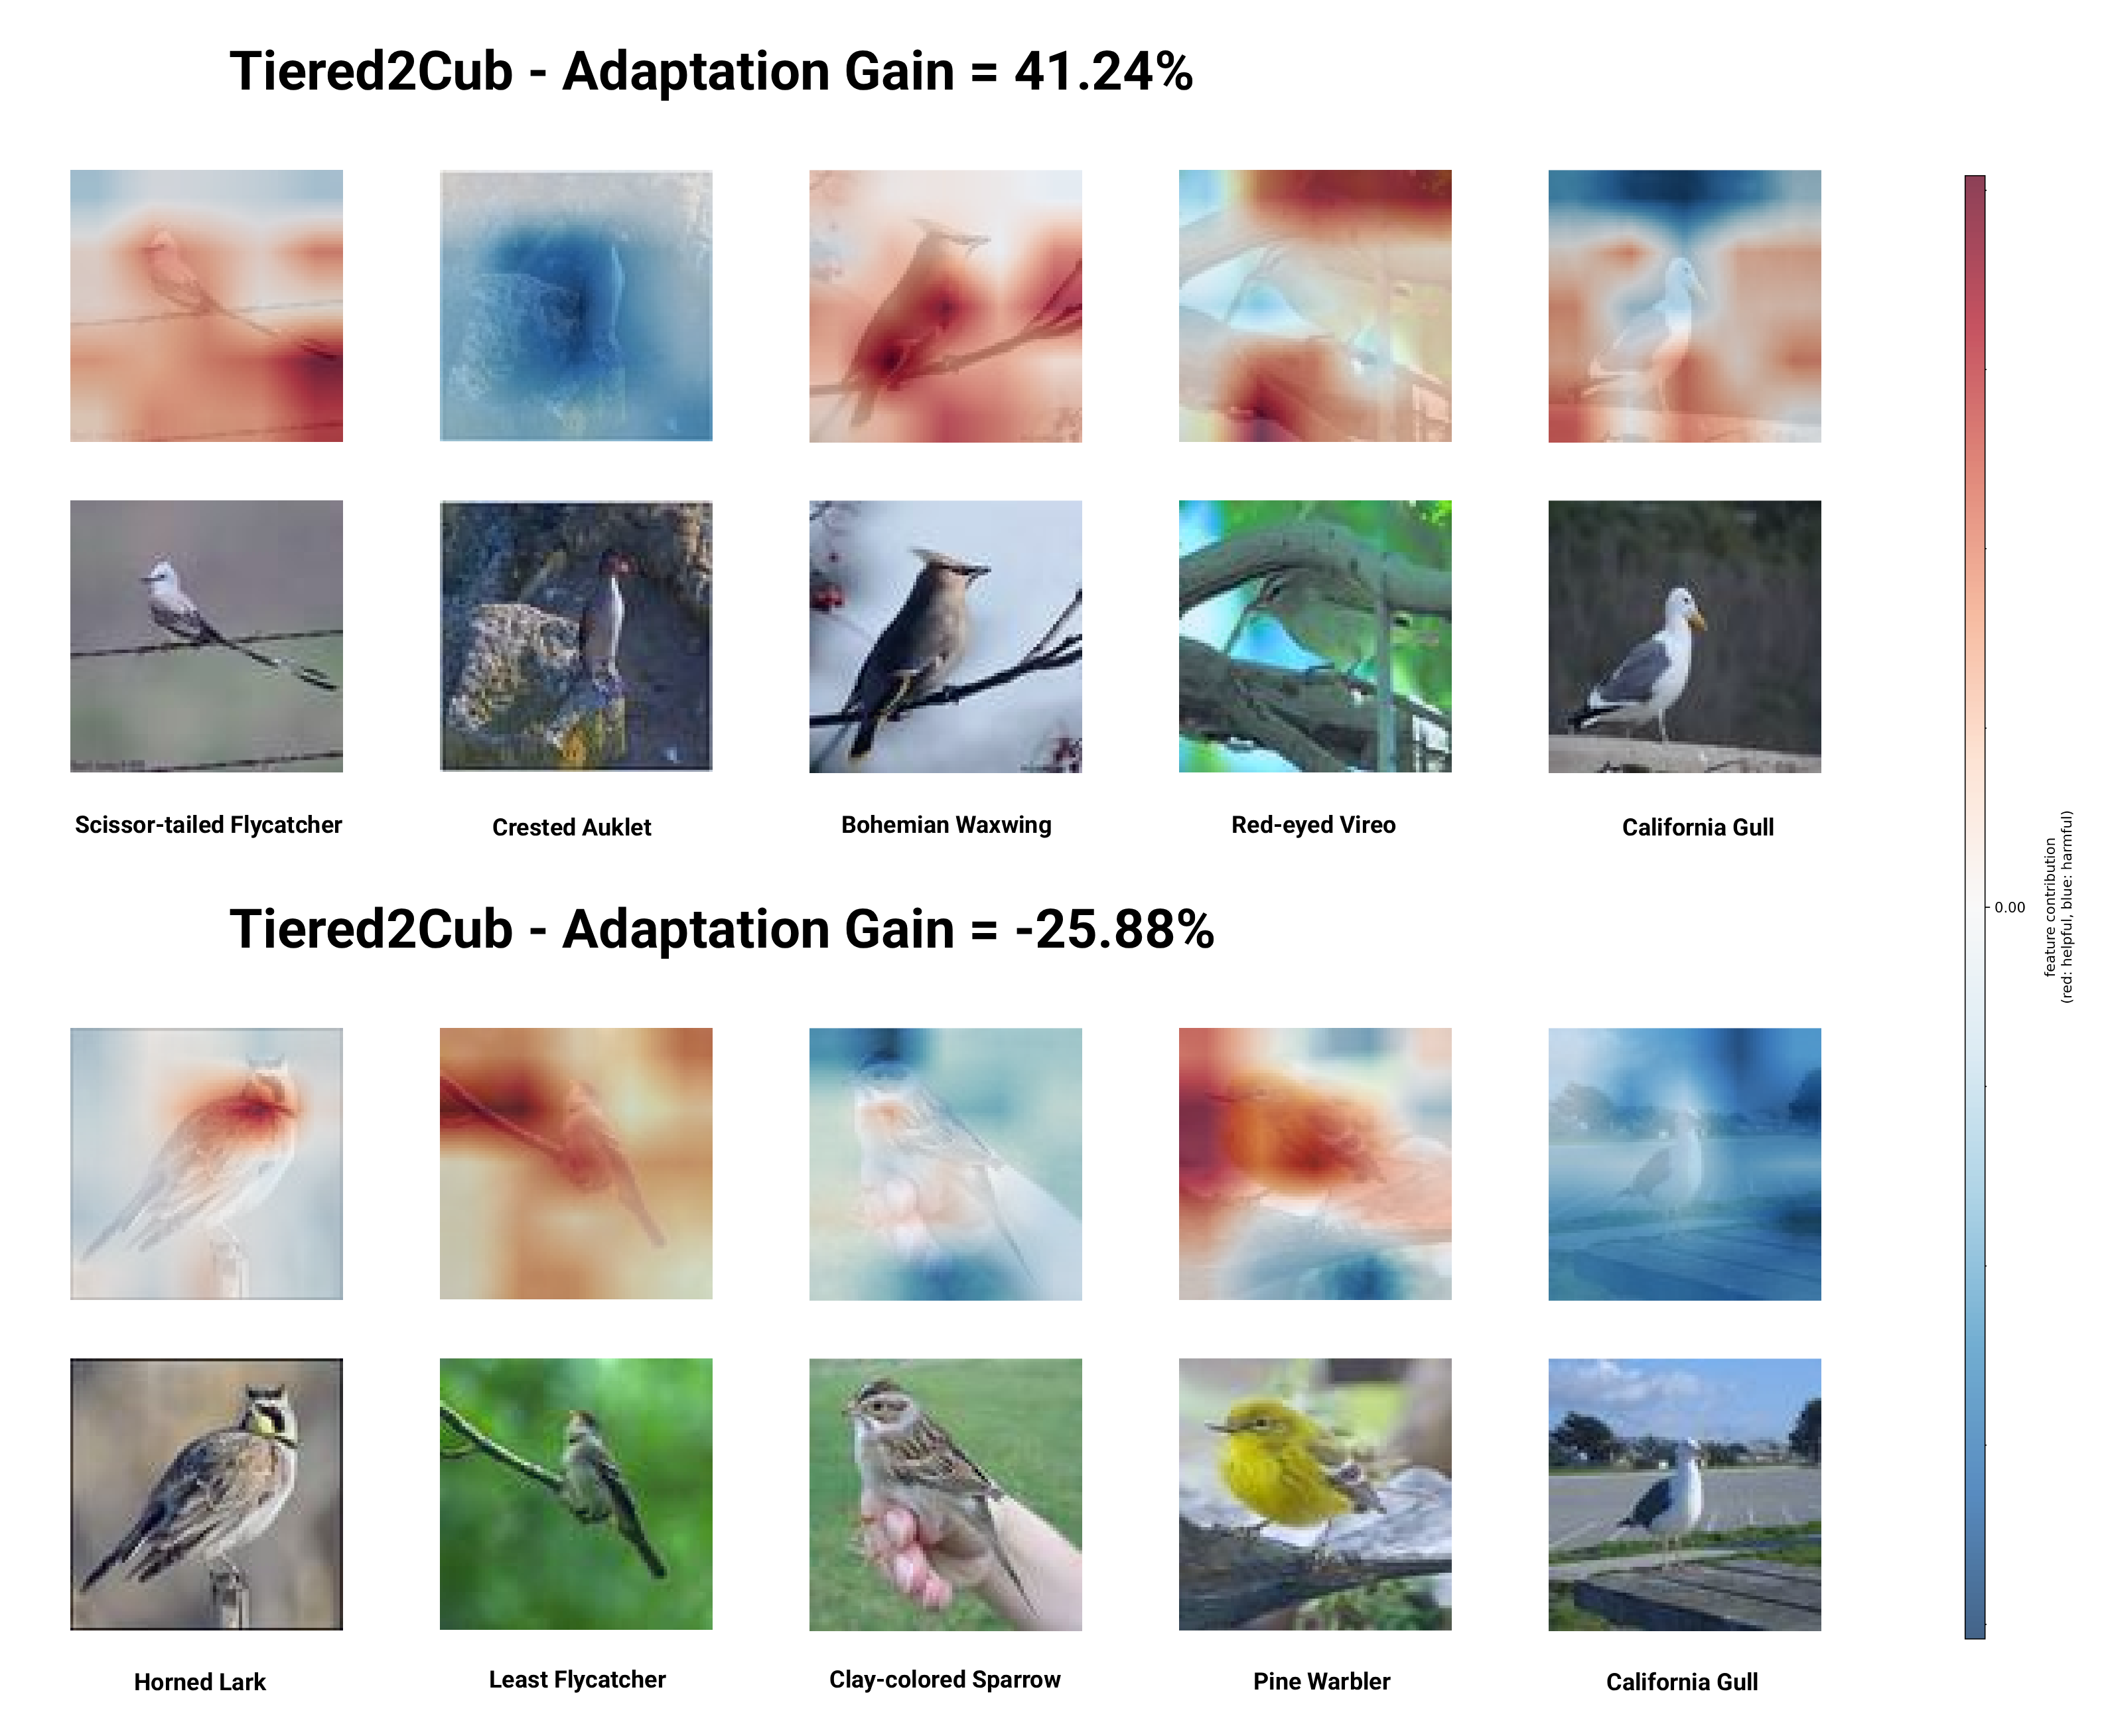
\includegraphics[width=0.95\linewidth]{figures/tiered2cub_lmag.png}
    \caption{$\PhiFama$ on the most positive- (top) and most negative-transfer (bottom) tiered2cub tasks (red: helpful, blue: harmful). Positive cases lock onto discriminative body/plumage regions; negative cases spend their attribution budget on background, occlusion, or artifacts instead of the bird.}
    \label{fig:case_study}
\end{figure*}

\Cref{fig:case_study} shows the extreme tasks from \Cref{fig:delta_m_dist} (mini2cub counterparts in the supplementary). We inspected the tasks at both tails of the $\Delta M$ distribution in \Cref{fig:delta_m_dist}, and three patterns recur among them. \textbf{(1) Contextual bias.} On plain backgrounds, positive-transfer maps lock tightly onto the bird itself (\emph{Bohemian Waxwing}) or a discriminative body part (\emph{Horned Lark}'s head plumes); when the subject is visually indistinct or partly occluded, red shifts onto surrounding branches or foliage instead (\emph{Scissor-tailed Flycatcher}, \emph{Crested Auklet}) -- i.e.\ the backbone falls back on background correlations exactly when the object itself offers a weak signal, the mechanism negative transfer is hypothesized to exploit. \textbf{(2) Artifact sensitivity.} Blue attribution consistently lands on non-biological confounds: color noise (\emph{Red-eyed Vireo}), camouflage-like clutter (\emph{Crested Auklet}), or a human hand holding the bird (\emph{Clay-colored Sparrow}) -- evidence that $\PhiFama$ tracks image-specific content rather than a class-level template, corroborating \Cref{sec:sanity}. Tellingly, \emph{California Gull} appears once in each extreme with near-opposite attribution structure, so the same class label is not what determines the map. \textbf{(3) Spatial bleeding.} For small subjects (\emph{Scissor-tailed Flycatcher}, both extremes), attribution leaks past the object boundary into the background -- the qualitative counterpart of \Cref{tab:biadt}'s wide \biadt margins, and, like them, a resolution artifact of Conv4's coarse final feature grid rather than a sign error.

We report contextual bias as a case-study observation, not yet a population-level statistic: \Cref{fig:case_study} and its supplementary counterpart cover the extreme tasks we selected for inspection, not all 600. A direct quantitative test is a natural next step and needs no new machinery -- CUB-200-2011 ships a bounding box per image, so the \emph{object sign-agreement rate}, the fraction of $\PhiFama$'s positive mass that falls inside the box versus outside it, averaged over all 600 tasks and correlated against $\Delta M$, would turn "background reliance co-occurs with negative transfer" from a pattern we observed in extreme cases into a population-level statistic.
